% ===== CHAPTER 4 =====
\chapter{谐振子}
\label{chap:4}
    我们将在第 13.2 节中看到,气相分子的能量可以近似为平动、转动、振动和电子能量之和。电子能量的计算将在第 13 章至第 17 章中讨论。平动能是分子作为一个整体在容纳物质的容器空间中的运动动能。平动能级可视为三维空间中粒子的能级(第 3.5 节)。二原子(双原子)分子的转动能级可以用刚性转子的转动能级来近似表示,第 6.4 节将对此进行讨论。双原子分子的最低几个振动能级可以用谐振子的能级来近似表示(第 4.3 节),多原子分子的振动能可以用线性谐振子振动能之和来近似表示(第 15.12 节)。本章第 4.2 节将求解谐振子的薛定谔方程。作为初步介绍,第 4.1 节讨论了求解微分方程的幂级数解法,该方法用于求解谐振子的薛定谔方程。第 4.3 节讨论分子振动。第 4.4 节介绍了求一维薛定谔方程特征值和特征函数的数值方法。
\section{微分方程的幂级数解}
\label{sec:4.1 Power-Series Solutions of Differential Equations}
    到目前为止,我们只考虑了势能$V\left(x\right)$是常数的情况。这使得薛定谔方程成为一个具有常数系数的二阶线性齐次微分方程,我们知道如何求解这个方程。对于 $V$ 随 $x$ 变化的情况,一种有用的方法是尝试薛定谔方程的幂级数解法。\\
    \indent 为了说明这种方法,考虑微分方程
    \begin{equation}
        y^{\prime\prime}\left(x\right) + c^2 y\left(x\right) = 0
        \label{eq:4.1}
    \end{equation}
    其中$c^2>0$。当然,这个微分方程有常系数,但我们可以用幂级数法求解。让我们先用特征方程$s^2+c^2=0$来求解这个方程。特征方程的根是$s=\pm \mathrm{i}c$。回忆第 2.2 节中的工作[公式 (\ref{eq:2.10 schrödinger equation for particle between 0 and l}) 和 (\ref{eq:4.1}) 是相同的],当特征方程的根是纯虚数时,我们会得到三角函数形式的通解:
    \begin{equation}
        y\left(x\right) = A \cos\: cx + B \sin\: cx
        \label{eq:4.2}
    \end{equation}
    其中 $A$ 和 $B$ 是积分常量。式(\ref{eq:4.2})的另一种形式是
    \begin{equation}
        y = D \sin\left(cx+e\right)
        \label{eq:4.3}
    \end{equation}
    其中 $D$ 和 $e$ 是任意常数。利用两角之和的正弦公式,我们可以证明 (\ref{eq:4.3}) 等价于 (\ref{eq:4.2})。\\
    \indent 现在让我们用幂级数法来求解 (\ref{eq:4.1})。我们假设方程的解可以在$x=0$处展开成Taylor级数的形式(见问题:4.1),也就是说,我们假设
    \begin{equation}
        y\left(x\right) = \sum_{n=0}^{\infty}a_nx^n = a_0 + a_1 x + a_2 x^2 + a_3 x^3 + \cdots
        \label{eq:4.4}
    \end{equation}
    其中 $a$ 为常数系数,有待确定,以使式 (\ref{eq:4.1}) 成立。对式(\ref{eq:4.4})求导,有
    \begin{equation}
        y^{\prime}\left(x\right) = a_1 + 2a_2 x + 3a_3 x^2 + \cdots = \sum_{n=1}^{\infty}na_nx^{n-1}
        \label{eq:4.5}
    \end{equation}
    其中,我们假设该数列可以逐项求导(对于无穷级数来说,这并不总是正确的)。对于$y^{\prime\prime}$,我们有
    \begin{equation}
        y^{\prime\prime}\left(x\right) = 2a_2 + 3\left(2\right)a_3 x + \cdots = \sum_{n=2}^{\infty}n(n-1)a_nx^{n-2}
        \label{eq:4.6}
    \end{equation}
    将 (\ref{eq:4.6}) 和 (\ref{eq:4.4}) 代入 (\ref{eq:4.1}),得到
    \begin{equation}
        \sum_{n=2}^{\infty}n(n-1)a_nx^{n-2} + c^2\sum_{n=0}^{\infty}a_nx^n = 0
        \label{eq:4.7}
    \end{equation}
    我们想把 (\ref{eq:4.7}) 中的两个和合并起来。只要满足一定条件,我们就可以将两个无穷级数逐项相加,得到它们的和:
    \begin{equation}
        \sum_{j=0}^{\infty}b_jx^j + \sum_{j=0}^{\infty}c_jx^j = \sum_{j=0}^{\infty}(b_j+c_j)x^j
        \label{eq:4.8}
    \end{equation}
    要将 (\ref{eq:4.8}) 应用于 (\ref{eq:4.7}) 中的两个和,我们希望每个和的极限相同,$x$ 的幂相同。因此,我们改变了 (\ref{eq:4.7}) 中第一个和的下标,定义$k \equiv n-2$。极限$n = 2$到无穷大与$k = 0$到无穷大相对应,将$n=k+2$代入第一个和,有
    \begin{equation}
        \sum_{n=2}^{\infty}n\left(n-1\right)a_nx^{n-2} = \sum_{k=0}^{\infty}\left(k+2\right)\left(k+1\right)a_{k+2}x^k = \sum_{n=0}^{\infty}\left(n+2\right)\left(n+1\right)a_{n+2}x^n
        \label{eq:4.9}
    \end{equation}
    (\ref{eq:4.9}) 中的最后一个等式是有效的,因为求和指数是一个\textbf{虚拟变量}(dummy variable);我们用什么字母来表示这个变量没有区别。例如,求和$\sum_{i=1}^{3}c_ix^i$和$\sum_{m=1}^{3}c_mx^m$是相等的,因为它们只有求和指数不同。如果我们将这个求和展开就会更好理解:
    \begin{equation*}
        \sum_{i=1}^{3}c_ix_6 = c_1x^1 + c_2x^2 + c_3x^3, \quad \sum_{m=1}^{3}c_mx^m = c_1x^1 + c_2x^2 + c_3x^3
    \end{equation*}
    在 (\ref{eq:4.9}) 的最后一个等式中,我们只是将表示求和指数的符号从 $k$ 改为 $n$。定积分中的积分变量也是一个虚拟变量,因为定积分的值不受变量字母的影响:
    \begin{equation}
        \int_{a}^{b}f\left(x\right)dx = \int_{a}^{b}f\left(t\right)dt
        \label{eq:4.10}
    \end{equation}
    将式(\ref{eq:4.9}) 代入 (\ref{eq:4.7}),我们得到
    \begin{equation}
        \sum_{n=0}^{\infty}\left[\left(n+2\right)\left(n+1\right)a_{n+2}+c^2a_n\right]x^n = 0
        \label{eq:4.11}
    \end{equation}
    如果 (\ref{eq:4.11}) 对所有 $x$ 值都成立,那么 $x$ 的每个幂的系数都必须为零。为了说明这一点,请看方程
    \begin{equation}
        \sum_{j=0}^{\infty}b_jx^j = 0
        \label{eq:4.12}
    \end{equation}
    在式(\ref{eq:4.12}),令$x=0$,我们有$b_0=0$。将式(\ref{eq:4.12})左右两侧对$x$求导,则$b_1=0$。求$n$阶导数,令$x=0$,我们得到$b_n=0$。因此,从式(\ref{eq:4.11})中,我们有:
    \begin{equation}
        \left(n+2\right)\left(n+1\right)a_{n+2} + c^2 a_n = 0
        \label{eq:4.13}
    \end{equation}
    \begin{equation}
        a_{n+2} = -\frac{c^2}{\left(n+1\right)\left(n+2\right)}a_n
        \label{eq:4.14}
    \end{equation}
    方程(\ref{eq:4.14}) 是一个\textbf{递推关系式}(recursion relation),如果我们知道$a_0$的值,就能用式(\ref{eq:4.14})计算出$a_2$、$a_4$、$a_6$等的值。如果我们知道$a_1$的值,就能用式(\ref{eq:4.14})计算出$a_3$、$a_5$、$a_7$等的值。由于对$a_0$和$a_1$的选择没有限制,它们是任意常数,我们分别用$A$和$Bc$来表示:
    \begin{equation}
        a_0 = A, \quad a_1 = Bc
        \label{eq:4.15}
    \end{equation}
    则利用式(\ref{eq:4.14}),我们可以计算系数:
    \begin{equation*}
        a_0 = A, \quad a_2 = -\frac{c^2}{1 \cdot 2}A, \quad a_4 = \frac{c^4}{1 \cdot 2\cdot 3}A, \quad a_6 = -\frac{c^6}{6!}A, \quad \ldots
    \end{equation*}
    \begin{equation}
        a_{2k} = (-1)^k \frac{c^{2k}}{(2k)!}A, \quad k = 0, 1, 2, \ldots
        \label{eq:4.16}
    \end{equation}
    \begin{equation*}
        a_1 = Bc, \quad a_3 = -\frac{c^3}{2 \cdot 3}Bc, \quad a_5 = \frac{c^5}{2 \cdot 3 \cdot 4 \cdot 5}Bc, \quad a_7 = -\frac{c^7}{7!}Bc, \quad \ldots
    \end{equation*}
    \begin{equation}
        a_{2k+1} = (-1)^k \frac{c^{2k+1}}{(2k+1)!}B, \quad k = 0, 1, 2, \ldots
        \label{eq:4.17}
    \end{equation}
    根据式(\ref{eq:4.4})、 (\ref{eq:4.16}) 和 (\ref{eq:4.17}) 我们有
    \begin{equation}
        y = \sum_{n=0}^{\infty}a_nx^n = \sum_{n=0,2,4, \cdots}^{\infty}a_nx^n + \sum_{n=1,3,5, \cdots}^{\infty}a_nx^n
        \label{eq:4.18}
    \end{equation}
    \begin{equation}
        y = A\sum_{k=0}^{\infty}(-1)^k\frac{c^{2k}x^{2k}}{(2k)!} + B\sum_{k=0}^{\infty}(-1)^k\frac{c^{2k+1}x^{2k+1}}{(2k+1)!}
        \label{eq:4.19}
    \end{equation}
    (\ref{eq:4.19}) 中的两个级数是 $\cos\: cx$ 和 $\sin\: cx$ 的Taylor级数(问题:4.2)。因此,与式(\ref{eq:4.2}) 相同,我们有$y = \cos\: cx + \sin\: cx$。

\section{一维谐振子}
\label{sec:4.2 The One-Dimensional Harmonic Oscillator}
    在本节中,我们将通过求解一维谐振子的薛定谔方程来增加我们的量子力学知识。该系统是分子振动的重要模型。\\
    \\
    \textbf{经典力学的处理}\\
    在研究谐振子的波动力学之前,我们先回顾一下经典的处理方法。我们有一个质量为 $m$ 的单粒子,它被一个与粒子离原点的位移成正比的力吸引向原点:\\
    \begin{equation}
        F_x = -kx
        \label{eq:4.20}
    \end{equation}
    比例常数$k$称为\textbf{力常数}(force constant)。$F_x$是作用在粒子上的力在$x$方向上的分量。这也是这个一维问题中的总力。附着在弹簧上的质点遵守公式 (\ref{eq:4.20}),前提是弹簧没有从平衡位置大幅拉伸。\\
    \indent 由牛顿第二定律$F = ma$,我们有
    \begin{equation}
        - kx = m\frac{\mathrm{d}^2x}{\mathrm{d}t^2}
        \label{eq:4.21}
    \end{equation}
    其中$t$是时间。若令$c^2 = k/m$,则式(\ref{eq:4.21})与式(\ref{eq:4.1})相同。因此,其解为[将$c = \left(k/m\right)^{1/2}$代入式(\ref{eq:4.3})],有
    \begin{equation}
        x = A \sin\left(2\pi \nu t +b\right)
        \label{eq:4.22}
    \end{equation}
    其中$A$是\textbf{振幅}(the amplitude of vibration),$b$是积分常数,\textbf{振动频率}(vibration frequency)$\nu$是
    \begin{equation}
        \boxed{
            \nu = \frac{1}{2\pi}\left(\frac{k}{m}\right)^{1/2}
        }
        \label{eq:4.23}
    \end{equation}
    由于正弦函数的最大最小值分别为1和-1,相应地,满足式(\ref{eq:4.22}) 的$x$值在$A$和$-A$之间振荡。正弦函数的最小正周期为$2\pi$,则完成一次完整振荡所需的时间(称为\textbf{周期}(period))为正弦函数参数增加$2\pi$的时间。在$t+1/\nu$时刻,正弦函数的参数为$2\pi \nu \left(t+1/\nu\right) + b = 2\pi \nu t + 2\pi + b$,比$t$时刻的参数多了$2\pi$。因此,周期为$1/\nu$。周期的倒数就是单位时间内的振动次数(振动频率),因此频率为$\nu$。\\
    \indent 现在我们来考虑能量。在三维系统中,势能$V$与力的分量的关系为
    \begin{equation}
        \boxed{
            F_x = -\frac{\mathrm{d}V}{\mathrm{d}x}, \quad F_y = -\frac{\mathrm{d}V}{\mathrm{d}y}, \quad F_z = -\frac{\mathrm{d}V}{\mathrm{d}z}
        }
        \label{eq:4.24}
    \end{equation}
    方程(\ref{eq:4.24}) 是势能的定义。由于这是一个一维系统,我们有[式(\ref{eq:1.12 Potential energy in classical mechanics})]
    \begin{equation}
        F_x = -\frac{\mathrm{d}V}{\mathrm{d}x} = -kx
        \label{eq:4.25}
    \end{equation}
    对(\ref{eq:4.25})两边积分,我们得到$V = \int kx \mathrm{d}x = \frac{1}{2}kx^2 + C$,其中$C$是积分常数。势能总是有一个任意的附加常数。我们令$C = 0$,则
    \begin{equation}
        \boxed{
            V = \frac{1}{2}kx^2
        }
        \label{eq:4.26}
    \end{equation}
    将式(\ref{eq:4.23})带入,有
    \begin{equation}
        V = 2\pi^2 \nu^2 m x^2
        \label{eq:4.27}
    \end{equation}
    势能$V$的图象是一个抛物线。动能$T$可以由式(\ref{eq:4.22})对时间$t$求导得到:
    \begin{equation}
        T = \frac{1}{2}m\left(\frac{\mathrm{d}x}{\mathrm{d}t}\right)^2
        \label{eq:4.28}
    \end{equation}
    将$T$和$V$相加,我们得到了总能量:
    \begin{equation}
        E = T + V = \frac{1}{2}kA^2 = 2\pi\nu^2mA^2
        \label{eq:4.29}
    \end{equation}
    其中我们用到了$\sin^2\theta + \cos^2\theta = 1$。\\
    \indent 根据式(\ref{eq:4.22}),经典力学中的谐振子在$x=A$和$x=-A$之间振荡运动。这两点是运动的转折点。在这两点,粒子的速度为零,而在$x=0$处速度达到最大值,同时势能为零而动能最大。经典的谐振子在$x=A$和$x=-A$附近的运动会比在$x=0$附近花费更多的时间(速度最慢)。问题 4.18 计算了在不同位置找到经典谐振子的概率密度。(有趣的是,这个概率密度在转折点处变得无限大)\\
    \\
    \textbf{量子力学的处理}\\
    由式(\ref{eq:3.27})和(\ref{eq:4.27}),谐振子的哈密顿算符为
    \begin{equation}
        \hat{H} = -\frac{\hbar^2}{2m}\frac{\mathrm{d}^2}{\mathrm{d}x^2} + 2\pi^2 \nu^2 m x^2 = -\frac{\hbar^2}{2m}\left(\frac{\mathrm{d}^2}{\mathrm{d}x^2} - \alpha^2x^2\right)
        \label{eq:4.30}
    \end{equation}
    其中,为了书写方便,我们定义了$\alpha$为
    \begin{equation}
        \alpha \equiv 2\pi\nu m/\hbar
        \label{eq:4.31}
    \end{equation}
    乘上$2m/\hbar^2$后,薛定谔方程$\hat{H}\psi = E\psi$变为
    \begin{equation}
        \frac{\mathrm{d}^2\psi}{\mathrm{d}x^2} + \left(2mE\hbar^{-2}-\alpha^2x^2\right)\psi = 0
        \label{eq:4.32}
    \end{equation}
    现在我们可以尝试求得 (\ref{eq:4.32}) 的幂级数解。如果我们现在考虑具有式(\ref{eq:4.4})形式的$\psi$幂级数,我们会发现它推出了一个三项递推关系,这比式 (\ref{eq:4.14}) 这样的两项递推关系更难处理。因此,我们修改 (\ref{eq:4.32}) 的形式,以便在尝试幂级数解时能得到两项的递推关系。能实现这一目的的替代方法(见问题 4.22)是$f\left(x\right) \equiv \mathrm{e}^{\alpha x^2/2}\psi\left(x\right)$。因此,
    \begin{equation}
        \psi = \mathrm{e}^{-\alpha x^2/2}f\left(x\right)
        \label{eq:4.33}
    \end{equation}
    这个方程只是定义了一个新函数$f\left(x\right)$,取代 $\psi\left(x\right)$ 作为未知函数来求解。(我们可以在微分方程中进行任何替换)对式(\ref{eq:4.33})两边求导两次,得到
    \begin{equation}
        \psi^{\prime\prime} = \mathrm{e}^{-\alpha x^2/2}\left(f0-2\alpha xf^{\prime} - \alpha f + \alpha^2x^2f\right)
        \label{eq:4.34}
    \end{equation}
    将(\ref{eq:4.34})和(\ref{eq:4.33})代入(\ref{eq:4.32}),我们得到
    \begin{equation}
        f^{\prime\prime}\left(x\right) - 2\alpha x f^{\prime}\left(x\right) + \left(2mE\hbar^{-2} - \alpha\right)f\left(x\right) = 0
        \label{eq:4.35}
    \end{equation}
    现在我们可以尝试幂级数解。假设
    \begin{equation}
        f\left(x\right) = \sum_{n=0}^{\infty}c_nx^N
        \label{eq:4.36}
    \end{equation}
    假设可以对式(\ref{eq:4.36})逐项求导,我们有
    \begin{equation}
        f^{\prime}\left(x\right) = \sum_{n=1}^{\infty}nc_nx^{n-1} = \sum_{n=0}^{\infty}nc_nx^{n-1}
        \label{eq:4.37}
    \end{equation}
    [式(\ref{eq:4.37})中第二个加和的第一项为零]。同样地,
    \begin{equation*}
        f^{\prime\prime}\left(x\right) = \sum_{n=2}^{\infty}n(n-1)c_nx^{n-2} = \sum_{j=0}^{\infty}(j+2)(j+1)c_{j+2}x^{j} = \sum_{n=0}^{\infty}(n+2)(n+1)c_{n+2}x^{n}
    \end{equation*}
    其中,我们令$j = n - 2$,然后将求和指数从 $j$ 改为 $n$ [见公式 (\ref{eq:4.9})]。代入 (\ref{eq:4.35}),我们得到
    \begin{equation*}
        \sum_{n=0}^{\infty}\left(n+2\right)\left(n+1\right)c_{n+2}x^n - 2\alpha \sum_{n=0}^{\infty}n c_n x^n + \left(2mE\hbar^{-2} - \alpha\right)\sum_{n=0}^{\infty}c_nx^n = 0
    \end{equation*}
    \begin{equation}
        \sum_{n=0}^{\infty}\left[(n+2)(n+1)c_{n+2} - 2\alpha n c_n + \left(2mE\hbar^{-2} - \alpha\right)c_n\right]x^n = 0
        \label{eq:4.38}
    \end{equation}
    令$x^n$的系数为零[与式(\ref{eq:4.11})一致],我们得到
    \begin{equation}
        c_{n+2} = \frac{\alpha + 2\alpha n - 2mE\hbar^2}{(n+1)(n+2)}c_n
        \label{eq:4.39}
    \end{equation}
    这正是我们想要的两项递推关系。式(\ref{eq:4.39})与式(\ref{eq:4.14})类似,知道了$c_n$的值,就可以计算出$c_{n+2}$的值。因此,我们有了两个任意常数$c_0$和$c_1$。如果我们令$c_1=0$,那么我们将得到一个只包含 $x$ 的偶数次幂乘以指数因子的幂级数作为解:
    \begin{equation}
        \psi = \mathrm{e}^{-\alpha x^2/2}f\left(x\right) = \mathrm{e}^{-\alpha x^2/2}\sum_{n=0,2,4,\cdots}^{\infty}c_{n}x^{n} = \mathrm{e}^{-\alpha x^2/2}\sum_{l=0}^{\infty}c_{2l}x^{2l}
        \label{eq:4.40}
    \end{equation}
    如果我们令$c_0=0$,那么我们将得到另一个独立的解:
    \begin{equation}
        \psi = \mathrm{e}^{-\alpha x^2/2}f\left(x\right) = \mathrm{e}^{-\alpha x^2/2}\sum_{n=1,3,5,\cdots}^{\infty}c_{n}x^{n} = \mathrm{e}^{-\alpha x^2/2}\sum_{l=0}^{\infty}c_{2l+1}x^{2l+1}
        \label{eq:4.41}
    \end{equation}
    薛定谔方程的通解为上述两个独立解的线性组合:
    \begin{equation}
        \psi = A\mathrm{e}^{-\alpha x^2/2}\sum_{l=0}^{\infty}c_{2l+1}x^{2l+1} + B\mathrm{e}^{-\alpha x^2/2}\sum_{l=0}^{\infty}c_{2l}x^{2l}
        \label{eq:4.42}
    \end{equation}
    其中 $A$ 和 $B$ 是任意常数。\\
    \indent 现在我们必须看看波函数的边界条件是否会对解法产生任何限制。为了了解这两个无穷级数在$x$充分大时的表现,我们要考察每个级数中连续系数的比值。在第二个级数中,$x^{2l+2}$与$x^{2l}$的比值为[在(\ref{eq:4.39})中令$n=2l$]:
    \begin{equation*}
        \frac{c_{2l+2}}{c_{2l}} = \frac{\alpha + 4\alpha l - 2mE\hbar^2}{(2l+1)(2l+2)}
    \end{equation*}
    假设对于较大的 $x$ 值,级数中的后项是主要项,那么我们就来看看对于较大的 $l$ 值,这一比值是多少:
    \begin{equation}
        \frac{c_{2l+2}}{c_{2l}} \sim \frac{4\alpha l}{4l^2} = \frac{\alpha}{l} \quad \text{当}l\text{很大时}
        \label{eq:4.43}
    \end{equation}
    在(\ref{eq:4.39})中令$n=2l+1$,我们发现,当 $l$ 较大时,第一个序列中连续系数的比值也是 $\alpha/l$。 现在考虑函数 $\mathrm{e}^{\alpha x^2}$ 的幂级数展开。(问题 4.3)
    \begin{equation}
        \mathrm{e}^{z} = \sum_{n=0}^{\infty}\frac{z^n}{n!} = 1 + z + \frac{z^2}{2!} + \cdots
        \label{eq:4.44}
    \end{equation}
    我们有
    \begin{equation*}
        \mathrm{e}^{\alpha x^2} = 1 + \alpha x^2 + \cdots + \frac{\alpha ^l x^{2l}}{l!} + \frac{\alpha ^{l+1} x^{2l+2}}{(l+1)!} + \cdots
    \end{equation*}
    在该级数中,$x^{2l+2}$和$x^{2l}$的系数比为
    \begin{equation*}
        \frac{\alpha^{l+1}}{\left(l+1\right)!} \div \frac{\alpha^l}{l!} = \frac{\alpha}{l+1} \sim \frac{\alpha}{l} \quad \text{当}l\text{很大时}
    \end{equation*}
    因此,解 (\ref{eq:4.42}) 中每个无穷级数的连续系数比与$l$很大时的级数$\mathrm{e}^{\alpha x^2}$相同。因此,我们可以得出结论:当$x$很大时,每个级数的行为都与 $\mathrm{e}^{\alpha x^2}$ 相同。[这不是一个严格的证明。H. A. Buchdahl, Am. J. Phys. J. Phys., 42, 47 (1974); see also M. Bowenand J. Coster, Am. J. Phys., 48, 307 (1980)]\\
    \indent 如果每个级数的行为都与 $\mathrm{e}^{\alpha x^2}$ 相同,那么当 $x$ 很大时,$\psi$ 的行为也将与 $\mathrm{e}^{\alpha x^2}$ 相同。当$x$趋于无穷时,波函数的值将趋于无穷大,就不满足波函数平方可积的要求。如果我们可以将级数在某一项打断,使得级数的后续项为零,那么因子$\mathrm{e}^{\alpha x^2}$就能保证在$x$趋于无穷时,$\psi$的值趋于零。(使用L' Hopital法则,显然当$x \to \infty$时,有$x^p\mathrm{e}^{-\alpha x^2} \to 0$,$p$为任意有限次幂)若想让级数在某一有限项后被打断,则当$n$为某个值时必须有递推公式(\ref{eq:4.39})中$c_n$的系数为零,记$n=v$。这就使得$c_{v+2}$、$c_{v+4}$$\cdots$等全为零。而式(\ref{eq:4.42})中的一个级数将具有有限项。在递推关系 (\ref{eq:4.39}) 中,有一个量的值尚未确定,但可以通过调整,使$c_v$消失。这个量就是能量$E$。在(\ref{eq:4.39}中)令$c_v$的系数为零,对$\alpha$使用式(\ref{eq:4.31}),我们有
    \begin{equation*}
        \alpha + 2\alpha v - 2mE\hbar^{-2} = 0
    \end{equation*}
    \begin{equation*}
        2mE\hbar^{-2} = \left(2v+1\right)2\pi\nu m/\hbar^{-1}
    \end{equation*}
    \begin{equation}
        \boxed{
            E = \left(v+\frac{1}{2}\right)h\nu, \quad v = 0, 1, 2, \ldots
        }
        \label{eq:4.45}
    \end{equation}
    \begin{figure}[h!]
        \centering
        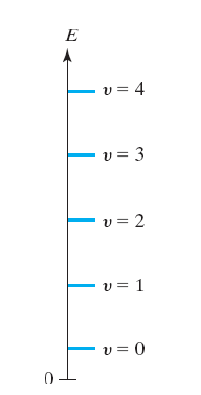
\includegraphics[width=0.2\textwidth]{Figures/4.1.png}
        \caption{\text{一维谐振子最低的五个能级图}}
        \label{fig:4.1}
    \end{figure}
    谐振子定态能级 (\ref{eq:4.45}) 间距相等(图\ref{fig:4.1})。不要混淆量子数$v$(vee)和振动频率$\nu$(nu)。\\
    \indent 将(\ref{eq:4.45})代入(\ref{eq:4.39}),我们得到
    \begin{equation}
        c_{n+2} = \frac{2\alpha \left(n-v\right)}{(n+1)(n+2)}c_n
        \label{eq:4.46}
    \end{equation}
    \indent 根据(\ref{eq:4.45})对能量进行量子化,我们已经使其中一个级数在有限项后被打断。为了消除 (\ref{eq:4.42}) 中的另一个无穷级数,我们必须将与之相乘的任意常数设为零。这样,根据 $v$ 是偶数还是奇数,波函数就是只包含 $x$ 的偶次或奇次幂的有限幂级数的 $\mathrm{e}^{-\alpha x^2/2}$ 倍。在该级数中,由于我们选择的能量$E$使得$c_{v+2}$、$c_{v+4}$,$\cdots$全消失,则$x$的最高次幂为$v$。因此,波函数(\ref{eq:4.42})的形式为
    \begin{equation}
        \psi_v = 
        \begin{cases}
            \mathrm{e}^{-\alpha x^2/2}\left(c_0+c_2x^2+ \cdots + c_vx^v\right), & \text{当} v \text{为偶数时} \\
            \mathrm{e}^{-\alpha x^2/2}\left(c_1x+c_3x^3+ \cdots + c_vx^v\right), & \text{当} v \text{为奇数时}
        \end{cases}
        \label{eq:4.47}
    \end{equation}
    其中任意常数$A$与$B$可被包含在$c_0$和$c_1$中,因此可以略去。$c_0$和$c_1$之后的系数可以通过递推关系式(\ref{eq:4.46})计算得到。由于量子数$v$出现在了递推关系中,对于不同的$v$值,我们可以得到一组不同的系数$c_i$。例如,$\psi_4$中的$c_2$与$\psi_2$中的$c_2$是不同的。
    \begin{figure}[h!]
        \centering
        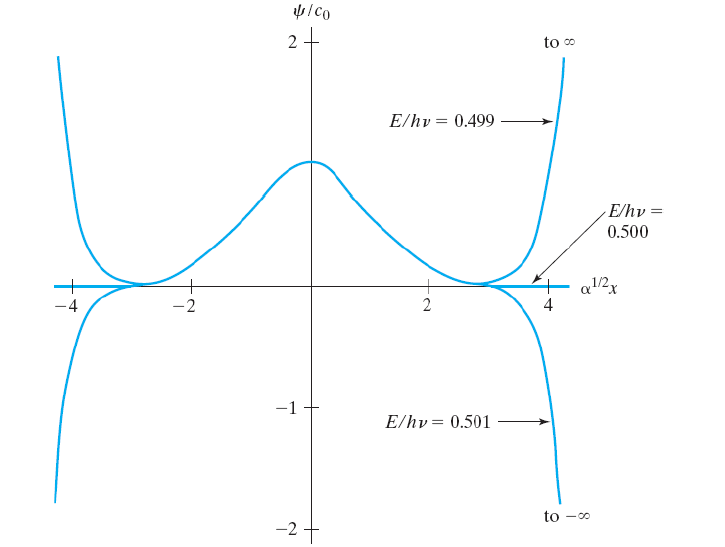
\includegraphics[width=0.75\textwidth]{Figures/4.2.png}
        \caption{
            \centering\parbox{\linewidth}{
                \centering
                当 $E = 0.499h\nu$、$E = 0.500h\nu$ 和 $E = 0.501h\nu$ 时,\\
                谐振子薛定谔方程的解只包含 $x$ 的偶次幂。\\
                在 $x = 0$ 附近的区域,三条曲线几乎重合。\\
                当 $|\alpha^{1/2} x| > 3$ 时,$E = 0.500h\nu$ 的曲线几乎与 $x$ 轴重合。
            }
        }
        \label{fig:4.2}
    \end{figure}\\
    \indent 与盒中粒子一样,波函数必须是品优波函数的要求迫使我们将能量量子化。对于不满足式(\ref{eq:4.45})的能量,$\psi$不是平方可积的。例如,图\ref{fig:4.2}显示了能量分别满足$E = 0.499h\nu$、$E = 0.500h\nu$和$E = 0.501h\nu$。当 $E = 0.500h\nu$ 时,式(\ref{eq:4.40})中的$\psi$,其中我们用到了递推关系(\ref{eq:4.39})来计算系数$c_n$(另见问题4.23)。图\ref{fig:4.2}显示了这些曲线在$\alpha^{1/2}x$附近区域的放大图。\\
    \indent 谐振子的基态能量不为零。这个能量$\frac{1}{2}h\nu$被称为\textbf{零点能量}(zero-point energy)。这是在绝对零度的温度下,谐振子集合中谐振子的振动能量。零点能可以由不确定性关系来理解。如果最低态的能量为零,那么它的势能和动能(均为非负值)都必须为零。动能为零则意味着动量也为零,那么$\Delta p_x = 0$。势能为零则意味着粒子始终处于原点,则$\Delta x = 0$。但我们不能同时让$\Delta p_x = 0$和$\Delta x = 0$,因此,基态能量必须大于零。零点能(ZPE)的定义为$E_{ZPE}=E_{gs} - V_{min}$,其中$E_{gs}$是基态能量,$V_{min}$是势能的最小值。
    \begin{figure}[h!]
        \centering
        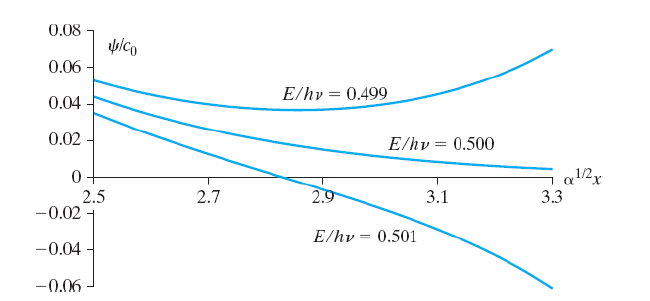
\includegraphics[width=0.75\textwidth]{Figures/4.3.png}
        \caption{
            图\ref{fig:4.2}在$\alpha^{1/2}x$附近区域的放大图。
        }
        \label{fig:4.3}
    \end{figure}\\
    \\
    \textbf{偶函数和奇函数}\\
    在详细考察波函数之前,我们先定义奇函数和偶函数。如果函数$f\left(x\right)$
    \begin{equation}
        \boxed{
            f\left(-x\right) = f\left(x\right)
        }
        \label{eq:4.48}
    \end{equation}
    则称$f\left(x\right)$为\textbf{偶函数}(even function)。因为$\left(-x\right)^2 = x^2$和$\mathrm{e}^{-b\left(x^2\right)} = \mathrm{e}^{-b\left(-x^2\right)}$,所以$x^2$和$\mathrm{e}^{bx^2}$均是偶函数。偶函数的图象关于$y$轴对称(例如,见图\ref{fig:4.4}a)。因此,对于偶函数,有
    \begin{equation}
        \boxed{
            \int_{-a}^{+a}f\left(x\right)\mathrm{d}x = 2\int_{0}^{a}f\left(x\right)\mathrm{d}x
        }
        \label{eq:4.49}
    \end{equation}
    如果$g\left(x\right)$满足
    \begin{equation}
        \boxed{
            g\left(-x\right) = -g\left(x\right)
        }
        \label{eq:4.50}
    \end{equation}
    则称$g\left(x\right)$为\textbf{奇函数}(odd function)。例如$x$、$1/x$和$x^3\mathrm{e}^{x^2}$。在式(\ref{eq:4.50})中,令$x=0$,若$g\left(0\right)$存在且为单值,则$g\left(0\right) = 0$。奇函数的图形大致如图\ref{fig:4.4} b 所示。由于 $y$ 轴一侧的正贡献会被另一侧相应的负贡献抵消,我们可以得出:对于奇函数,有
    \begin{equation}
        \boxed{
            \int_{-a}^{+a}g\left(x\right)\mathrm{d}x = 0
        }
        \label{eq:4.51}
    \end{equation}
    \begin{figure}[h!]
        \centering
        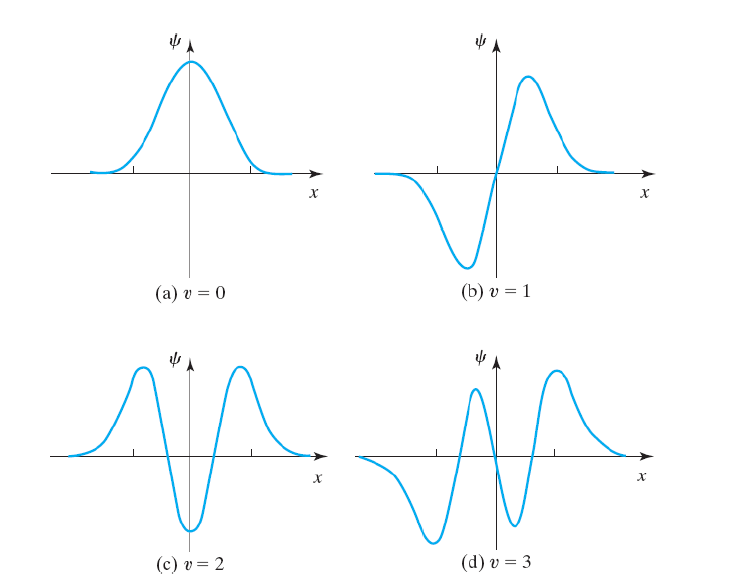
\includegraphics[width=0.75\textwidth]{Figures/4.4.png}
        \caption{
                \centering\parbox{\linewidth}{
                \centering
                谐振子波函数。\\
                所有图形使用相同的比例尺。$x$ 轴上标记的点为$\alpha^{1/2} x=\pm 2$。
            }
        }
        \label{fig:4.4}
    \end{figure}\\
    很容易证明,两个偶函数或两个奇函数的乘积是偶函数,而一个偶函数和一个奇函数的乘积是奇函数。\\
    \\
    \textbf{谐振子波函数}\\
    \indent 式(\ref{eq:4.47})中的指数部分$\mathrm{e}^{-\alpha x^2/2}$是偶函数。若$v$是偶数,则多项式因子只包含$x$的偶次幂,使得$\psi_v$是偶函数。若$v$是奇数,则多项式因子只包含$x$的奇次幂,使得$\psi_v$是一个奇函数和一个偶函数的乘积,为奇函数。每一个谐振子状态方程$\psi$都是一个奇函数或偶函数,取决于$v$的奇偶性。在第\ref{sec:7.5 Parity}节中,我们将看到:当势能函数$V$是偶函数时,非简并能级的波函数一定是奇函数或偶函数。\\
    \indent 现在,我们找到了最低三个能级波函数的显式。对于$v=0$的基态,式(\ref{eq:4.47})给出
    \begin{equation}
        \psi_0 = c_0\mathrm{e}^{-\alpha x^2/2}
        \label{eq:4.52}
    \end{equation}
    其中$\psi$的下标表示量子数$v$。通过归一化,我们可以求出$c_0$:
    \begin{equation*}
        1 = \int_{-\infty}^{\infty}\left|c_0\right|\mathrm{e}^{-\alpha x^2}\mathrm{d}x = 2\left|c_0\right|^2\int_{0}^{\infty}\mathrm{e}^{-\alpha x^2}\mathrm{d}x
    \end{equation*}
    其中,我们用到了式(\ref{eq:4.49})。使用附录中的积分(A.9),我们有$\left|c_0\right| = \left(\alpha/\pi\right)^{1/4}$。因此,如果我们选择令归一化常数的相位为零,则基态波函数为
    \begin{equation}
        \psi_0 = \left(\alpha / \pi\right)^{1/4}\mathrm{e}^{-\alpha x^2 /2}
        \label{eq:4.53}
    \end{equation}
    波函数 (\ref{eq:4.53}) 是一个高斯函数(图\ref{fig:4.4}a)。\\
    \indent 对于状态$v=1$,式(\ref{eq:4.47})给出
    \begin{equation}
        \psi_1 = c_1x\mathrm{e}^{-\alpha x^2 / 2}
        \label{eq:4.54}
    \end{equation}
    使用(A.10)进行归一化,我们有
    \begin{equation}
        \psi_1 = \left(4\alpha^3 / \pi\right)^{1/4}x\mathrm{e}^{-\alpha x^2 / 2}
        \label{eq:4.55}
    \end{equation}
    图\ref{fig:4.4}b显示了$\psi_1$的图象。\\
    \indent 对于状态$v=2$,式(\ref{eq:4.47})给出
    \begin{equation*}
        \psi_2 = \left(c_0 + c_2x^2\right)\mathrm{e}^{-\alpha x^2 / 2}
    \end{equation*}
    将$v=2$代入(\ref{eq:4.46}),我们有
    \begin{equation*}
        c_2 = \frac{2\alpha \left(-2\right)}{1\cdot2}c_0 = -2\alpha c_0
    \end{equation*}
    因此,
    \begin{equation}
        \psi_2 = c_0\left(1-2\alpha x^2\right)\mathrm{e}^{-\alpha x^2 / 2}
        \label{eq:4.56}
    \end{equation}
    使用归一化解出$c_0$,我们有(问题4.10)
    \begin{equation}
        \psi_2 = \left(4\alpha^3 / \pi\right)^{1/4}\left(2\alpha x^2 - 1\right)\mathrm{e}^{-\alpha x^2 / 2}
        \label{eq:4.57}
    \end{equation}
    注意:$\psi_2$中的$c_0$和$\psi_0$中的$c_0$是不同的。\\
    \indent 波函数节点的个数与量子数$v$相同。可以证明(见《Messiah》,第 109-110 页):\textit{对于一维定态束缚态问题,若$\psi$处于基态,则边界点内部的节点数为零;而对于每一个连续的激发态,节点数都会增加一个。}\\
    \begin{figure}[h!]
        \centering
        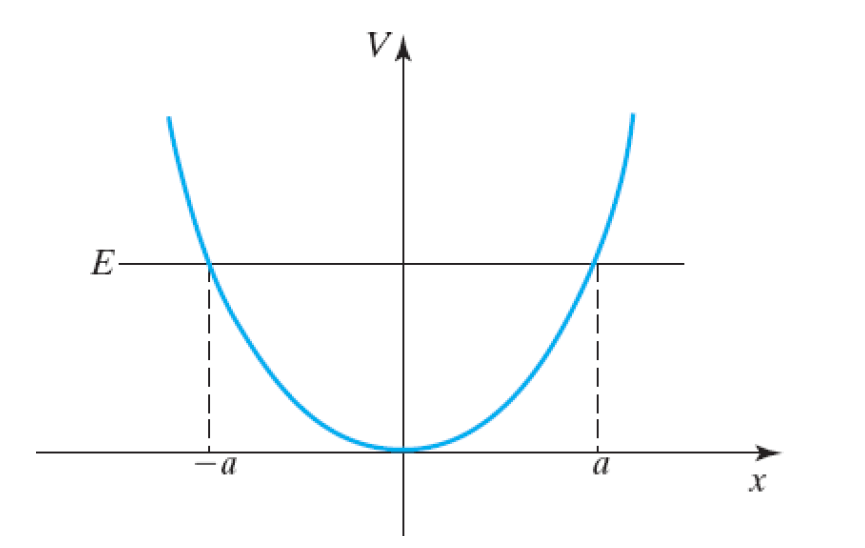
\includegraphics[width=0.65\textwidth]{Figures/4.5.png}
        \caption{
            谐振子的经典允许区域$-a \le x \le a$和禁阻区域$x > a$,$x < -a$
        }
        \label{fig:4.5}
    \end{figure}\\
    \indent 谐振子波函数中的多项式因子在数学中是众所周知的,被称为\textit{厄米多项式}(Hermite polynomials),是以一位法国数学家的名字命名的。(见问题 4.21)\\
    \indent 根据量子力学解法,在 $x$ 轴上的任何一点(节点除外)都有一定概率找到粒子。从经典角度讲,$E=T+V$,动能 $T$ 不能为负:$T \ge 0$。因此,$E-V = T \ge 0$则$V \le E$。势能 $V$ 是位置的函数,经典粒子被限制在 $V<E$ 的空间区域内。也就是说,势能不超过总能量。在图 (\ref{fig:4.5}) 中,标有 $E$ 的水平线表示谐振子的能量,抛物线表示势能 $\frac{1}{2}kx^2$。对于区域$x < -a$和$x > a$,我们有$V>E$,这些区域是\textbf{经典禁阻}(classical forbidden)的。\textbf{经典允许的区域}(classical allowed region) $-a \le x \le a$在图 (\ref{fig:4.5}) 中满足$V\le E$。\\
    \indent 在量子力学中,定态波函数不是算符$\hat{T}$或$\hat{V}$的本征函数,因此我们无法确定定态系统的动能或势能值。与经典力学的方程$E=T+V$和$T \ge 0$不同,在量子力学中我们有$\langle E \rangle = \langle T \rangle + \langle V \rangle$(问题6.35)和$\langle T \rangle \ge 0$(问题7.7),所以量子力学中满足$\langle V \rangle \le E$,但是我们不能写作$V \le E$,因此,粒子有一定概率在经典禁区($V>E$的区域)中被发现。\\
    \indent 如果说粒子可以在经典允许的区域之外被发现,我们似乎就允许它具有负动能。实际上,量子力学的观点并不存在悖论。为了验证粒子是否处于经典禁止区域,我们必须测量它的位置。这种测量会改变系统的状态(第 \ref{sec:1.3 The Uncertainty Principle} 和 \ref{sec:1.4 The Time-Dependent Schrödinger Equation} 节)。振子与测量仪器的相互作用会将足够的能量传递给振子,使其处于经典禁区。对 $x$ 的精确测量会给动量带来很大的不确定性,因此也会给动能带来很大的不确定性。\ref{sec:2.4 Particle in a Rectangular Potential Well} 节和 \ref{sec:2.5 Tunneling} 节讨论了经典禁区的穿透问题。\\
    \indent 一个定态谐振子满足$E = \left(v+\frac{1}{2}\right)h\nu$和$V=\frac{1}{2}kx^2 = 2\pi^2\nu^2mx^2$。因此,在经典允许的区域($V\le E$)有$2\pi^2\nu^2mx^2 \le \left(v+\frac{1}{2}\right)h\nu$,即$x^2 \le \left(v+\frac{1}{2}\right)h/2\pi^2\nu^2m = \left(2v+1\right)\alpha$,其中$\alpha \equiv 2\pi\nu m/\hbar$[式(\ref{eq:4.31})]。因此,谐振子的经典允许区域为$-\left(2v+1\right)^{1/2} \le \alpha^{1/2}x \le \left(2v+1\right)^{1/2}$。\\
    \indent 从图 (\ref{fig:4.4}) 中可以看出:\textit{$\psi$ 在经典允许区域中振荡,而在经典禁止区域则以指数形式下降到零。}我们之前在矩形势阱中看到过粒子的这种行为(第 \ref{sec:2.4 Particle in a Rectangular Potential Well} 节)。\\
    \indent 图 (\ref{fig:4.4}) 显示,当谐振子的能量逐渐升高时,$\psi$ 和 $\left|\psi\right|^2$ 的最大值往往离原点越来越远。由于离原点越远,势能$V = \frac{1}{2}kx^2$越大,平均势能$\langle V \rangle = \int_{-\infty}^{\infty}\left|\psi\right|^2V\mathrm{d}x$也会随着量子数的增加而增大。平均动能由$\langle T \rangle = -\left(\hbar^2/2m\right)\int_{-\infty}^{\infty}\psi^{\ast}\psi^{\prime\prime}\mathrm{d}x$给出。应用分部积分(问题7.7b),有$\langle T \rangle = \left(\hbar^2/2m\right)\int_{-\infty}^{\infty}\left|\mathrm{d}\psi/\mathrm{d}x\right|^2\mathrm{d}x$。量子数越大的状态中节点的数量越多,$\psi$ 的变化速度就越快,因此随着量子数的增加,$\langle T \rangle$也会增加。\\
    \indent 经典谐振子最有可能出现在运动转折点附近的区域,即振子运动速度最慢、$V$ 值较大的区域。相反,对于量子谐振子的基态,最有可能出现的区域是原点附近的区域。对于高振动量子数,人们会发现的外峰值大于原点附近的峰值,最可能的区域变成了经典转折点附近的区域,此时 $V$ 很大(见问题 4.18 )。这是对应原理(第 \ref{sec:2.2 Particle in a One-Dimensional Box} 节)的一个例子。\\
    \indent 量子谐振子的一些在线模拟可从以下网站获得:\url{www.phy.davidson.edu/StuHome/cabell_f/energy.html}(显示能级和波函数,并显示当能量从允许值改变时波函数如何发散);\url{www.falstad.com/qm1d/}(从顶部的下拉菜单中选择谐振子;双击底部的一个小圆圈以显示静止状态;显示能量、波函数、概率密度;$m$ 和 $k$ 可以改变);\url{demonrations.wolfram.com/HarmonicOscillatorEigenfunctions}(展示了$\left|\psi\right|^2$)。

\section{双原子分子的振动}
\label{sec:4.3 Vibrations of Diatomic Molecules}
    我们将在第 \ref{sec:13.1 The Born-Oppenheimer Approximation} 节中看到,在极好的近似条件下,我们可以分别处理分子中电子的运动和原子核的运动(这是由于原子核的质量要大得多)。首先想象原子核静止不动,然后求解电子能量 $U$ 的薛定谔方程($U$ 还包括核排斥能量)。对于二原子(双原子)分子,电子能量 $U$ 取决于原子核之间的距离 $R$,$U=U\left(R\right)$,而 $U$ 与 $R$ 的关系曲线则如图 13.1 所示。\\
    \indent 找到$U\left(R\right)$后,可以先解决核运动的薛定谔方程,使用$U\left(R\right)$作为核运动的势能函数。对于双原子分子,核薛定谔方程是一个双粒子方程。我们将在第 \ref{sec:6.3 Reduction of the Two-Particle Problem to Two One-Particle Problems} 节中看到,当双粒子系统的势能只取决于粒子之间的距离时,系统的能量是 (a) 整个系统在空间平动的动能和 (b) 粒子相对于彼此的内部运动能量之和。双粒子内部运动能量的经典表达式是粒子间相互作用的势能与假设粒子的动能之和,其中假设粒子的质量为$m_1m_2/\left(m_1+m_2\right)$($m_1$ 和 $m_2$ 分别是两个原子的质量),该粒子的坐标为一个粒子相对于另一个粒子的坐标。$m_1m_2/\left(m_1+m_2\right)$称为\textbf{约化质量}(reduced mass)$\mu$。\\
    \indent 二原子分子的内部运动包括\textbf{振动}和\textbf{转动},前者与两个原子核之间距离 $R$ 的变化相对应,后者与原子核连接线空间方向的变化相对应。通常可以近似地将振动和转动分开处理。转动能级见第 \ref{sec:6.4 The Two-Particle Rigid Rotor} 节。 此处我们考虑振动能级。\\
    \indent 双原子分子振动的薛定谔方程有一个质量为$m_1m_2/\left(m_1+m_2\right)$假设粒子的动能算符和一个由$U\left(R\right)$给出的势能项。如果我们将原点与图 13.1 中$U$曲线的最低点重合,并将该最低点的能量取为势能的零点,那么 $U(R)$ 曲线的下半部分将与具有适当力常数 $k$ 的谐振子的势能曲线几乎重合(见图 \ref{fig:4.6} 和问题 4.28)。$U(R)$ 曲线的最小值出现在\textbf{平衡核间距}(equilibrium distance)$R_e$的位置。在图 \ref{fig:4.6} 中,$x$ 是核间距与平衡核间距的偏差:$x \equiv R - R_e$。
    \begin{figure}[h!]
        \centering
        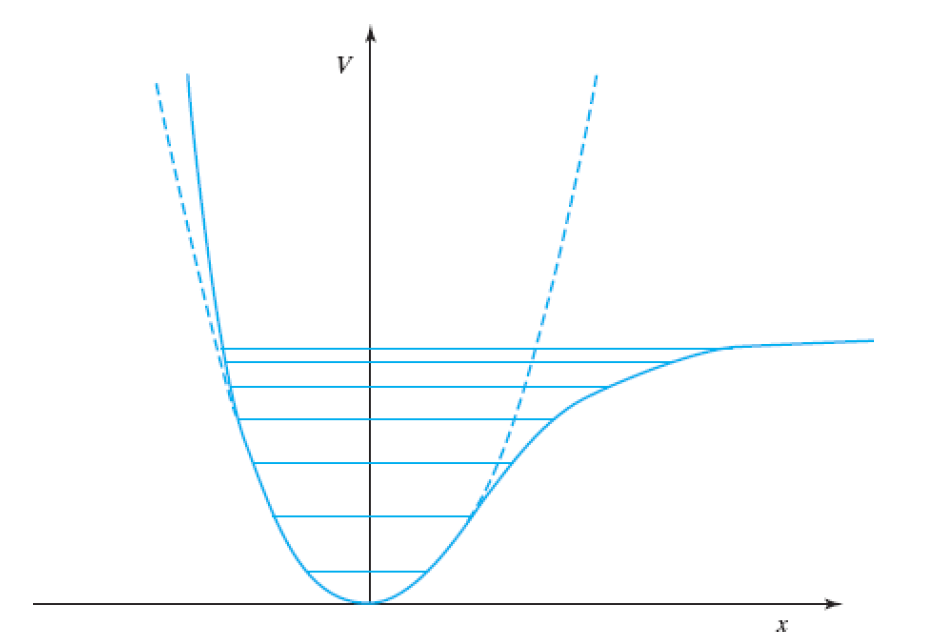
\includegraphics[width=0.7\textwidth]{Figures/4.6.png}
        \caption{
            \centering\parbox{\linewidth}{
                \centering
                二原子分子振动的势能(实线)和谐振子的势能(虚线)。\\
                图中还显示了二原子分子的束缚态振动能级。\\
                与谐振子相比,二原子分子只有有限数量的束缚振动能级。\\
            }
        }
        \label{fig:4.6}
    \end{figure}
    \\
    \indent 谐振子的力常数$k$在式(\ref{eq:4.26})中可以由$k = \mathrm{d}^2V /\mathrm{d}x^2$计算得到,在$R=R_e$处,谐振子曲线与$U(R)$曲线的下半部分几乎重合,所以分子的力常数$k = \left.\mathrm{d}^2U/\mathrm{d}R^2\right|_{R=R_e}$。(另见问题4.28)。\textit{核质量的差异对电子能量曲线 $U(R)$ 几乎没有影响,因此同一分子但由不同同位素取代的种类具有基本相同的力常数 $k$。}\\
    \indent 因此,我们预计二原子分子振动能级 $E_{vib}$ 的一个合理近似是谐振子振动能级;由式(\ref{eq:4.45})和式(\ref{eq:4.23}),有
    \begin{equation}
        \boxed{
            E_{vib} \approx \left(v+\frac{1}{2}\right)h\nu_e, \quad v = 0, 1, 2, \ldots
        }
        \label{eq:4.58}
    \end{equation}
    \begin{equation}
        \boxed{
            \nu_e = \frac{1}{2\pi}\left(\frac{k}{\mu}\right)^{1/2}, \quad \mu = \frac{m_1m_2}{m_1+m_2}, \quad k = \left.\frac{\mathrm{d}^2U}{\mathrm{d}R^2}\right|_{R=R_e}
        }
        \label{eq:4.59}
    \end{equation}
    其中$\nu_e$称为\textbf{简谐振动频率}(equilibrium or harmonic vibrational frequency)。这种近似方法最适用于较低的振动能级。随着$v$的增加,原子核位于远离其平衡间隔区域的时间更长。对于这些区域,势能大大偏离谐振子的势能,谐振子近似效果不佳。我们会发现:随着 $v$ 的增大,双原子分子的振动能级不是等距排列,而是越靠越近(图 \ref{fig:4.6})。最终,振动能量大到足以将双原子分子解离成互不结合的原子。与谐振子不同,双原子分子只有有限数量的束缚态振动能级。考虑到振动的非谐性,分子振动能的更精确表达式是
    \begin{equation}
        E_{vib} = \left(v+\frac{1}{2}\right)h\nu_e - \left(v+\frac{1}{2}\right)^2h\nu_e \chi_e
        \label{eq:4.60}
    \end{equation}
    其中\textit{非谐性常数}(anharmonicity constant)$\nu_e\chi_e$几乎在所有情况下都大于零。(\textit{译者注:一般认定$\chi_e$为非谐性常数?})\\
    \indent 使用含时薛定谔方程,我们可以发现(见第\ref{sec:9.9 Interaction of Radiation and Matter}节):当双原子分子暴露在电磁辐射下时,最有可能发生的振动跃迁是那些 $v$ 变化了 $\pm 1$ 的跃迁。此外,要吸收或发射电磁辐射,振动必须改变分子的偶极矩。因此,同核双原子分子(例如$\mathrm{H}_2$、$\mathrm{N}_2$)不能通过吸收或发射辐射实现振动能级之间的转换(这种转变可以发生在分子间碰撞中)。关系$E_{upper}-E_{lower} = h\nu$(其中$\nu$为辐射频率)、近似方程(\ref{eq:4.58})、吸收和发射辐射的\textbf{选律}(selection rule)$\Delta v = \pm 1$表明:一个振动频率为$\nu_e$的异核双原子分子将对近似为下式给出频率的辐射$\nu_{light}$有强烈吸收:
    \begin{equation}
        \nu_{light} = \left(E_2-E_1\right)/h \approx \left[\left(v_2+\frac{1}{2}\right)h\nu_e-\left(v_1+\frac{1}{2}\right)h\nu_e\right]/h = \left(v_2-v_1\right)\nu_e = \nu_E
        \label{eq:4.61}
    \end{equation}
    双原子分子$k$和$\mu$值的特性使得$\nu_{light}$通常位于光谱的红外区域。$\Delta v = 2,3,\cdots$的跃迁也会发生,但这些(称为\textit{泛频}(overtones))的吸收要比$\Delta v = 1$的跃迁弱得多。\\
    \indent 使用更准确的方程(\ref{eq:4.60}),有(问题4.27)
    \begin{equation}
        \nu_{light} = \nu_e - 2\nu_e\chi_e\left(v_1+1\right)
        \label{eq:4.62}
    \end{equation}
    其中$v_1$是较低能级的振动量子数,选律为$\Delta v = \pm 1$。\\
    \indent 热平衡系统中分子两个能级的布居数由\textbf{玻尔兹曼分布律}(Boltzmann distribution law)给出(见物理化学教材):
    \begin{equation}
        \boxed{
            \frac{N_i}{N_j} = \frac{g_i}{g_j} \mathrm{e}^{-(E_i-E_j)/kT}
        }
        \label{eq:4.63}
    \end{equation}
    其中能级$i$和$j$的能量分别为$E_i$和$E_j$,$g_i$和$g_j$是对应能级的简并度,$k$是玻尔兹曼常数,$T$是热力学温度。对于非简并能级,有$g_i=1$。\\
    \indent $\nu = \left(1/2\pi\right)\left(k/\mu\right)^{1/2}$的数量级使得在室温下,对于轻分子(例如$\mathrm{H}_2$、$\mathrm{HCl}$、$\mathrm{CO}$),只有$v=0$的振动能级是被显著占据的。对于重分子(例如$\mathrm{I}_2$),在室温下有一个或多个激发态振动能级被显著占据。\\
    \indent 极性双原子分子的振动吸收光谱包含$v= 0 \to 1$吸收带,很弱的泛频吸收带($v = 0\to 2, 0 \to 3, \cdots$),以及若$v>0$的能级也被显著占据,也有\textit{热带}(hot bands),例如$v = 1 \to 2$、$v = 1 \to 3$等。与特定振动跃迁相对应的每个波段都由几条紧密相连的线组成。每一条这样的线都对应于与振动状态变化同时发生的不同的转动状态变化。每一条线都是振动-转动跃迁的结果。\\
    \indent 光谱频率的国际单位为\textbf{赫兹}(hertz,Hz),定义
    为$1 \:\mathrm{Hz} \equiv 1 \:\mathrm{s}^{-1}$。通常使用的倍数有等于 $10^6$ 赫兹的兆赫兹(MHz)和等于 $10^9$ 赫兹的千兆赫兹(GHz)。红外(IR)吸收峰通常由\textbf{波数}(wavenumber)$\tilde{\nu}$给出,定义为
    \begin{equation}
        \boxed{
            \tilde{\nu} \equiv \frac{\nu}{c} = \frac{1}{\lambda}
        }
        \label{eq:4.64}
    \end{equation}
    其中$\lambda$是真空中辐射的波长。\\
    \indent 在谐振子近似中,多原子分子的量子力学能级为$E_{vib} = \sum i\left(v_i+\frac{1}{2}\right)h\nu_i$,其中$\nu_i$是分子每个正则振动模式的频率,$v_i$是对应第$i$个正则振动的量子数。每个振动量子数$v_i$的取值$0,1,2,\cdots$都与其他振动量子数的取值无关。一个具有$n$个原子的线性分子具有$3n-6$个正则振动模式,而一个具有$n$个原子的非线性分子具有$3n-5$个正则振动模式。\\
    \indent 为了由式(\ref{eq:4.59})计算折合质量$\mu$,我们需要知道每种同位素的质量。附录表 A.3 列出了一些常见同位素的相对原子质量。\\
    \begin{examplebox}
        \textbf{例题:}$^{12}\mathrm{C}^{16}\mathrm{O}$分子的最强红外吸收峰位于$\tilde{\nu} = 2140 \:\mathrm{cm}^{-1}$。计算该分子的力常数 $k$。请说明所做的近似计算。\\
        \\
        最强的红外吸收峰对应于$v = 0 \to 1$的跃迁。我们将分子振动近似为谐振子模型。由式(\ref{eq:4.61}),分子的平衡振动频率近似为
        \begin{equation*}
            \nu_e \approx \nu_{light} = \tilde{\nu}c = \left(2140 \:\mathrm{cm}^{-1}\right)\left(2.9979 \times 10^{10} \:\mathrm{cm/s}\right)  = 6.424 \times 10^{13} \:\mathrm{s}^{-1}
        \end{equation*}
        使用式(\ref{eq:4.59}),将$k$与$\nu_e$联系起来,我们需要折合质量$\mu = m_1m_2/\left(m_1+m_2\right)$。1 mol $^{12}\mathrm{C}$的质量为12 g,包含阿伏伽德罗常数($N_A$)个分子,则一个$^{12}\mathrm{C}$原子的质量为$\left(12 \: \mathrm{g} \right)/ \left(6.02214 \times 10^{23}\right)$。折合质量和力常数分别为
        \begin{equation*}
            \mu = \frac{12 \left(15.9949\right)\: g}{27.9949} \frac{1}{6.02214 \times 10^{23}} = 1.1385 \times 10^{-23} \:\mathrm{g}
        \end{equation*}
        \begin{equation*}
            k = 4\pi^2 \nu_e^2\mu = 4\pi^2 \left(6.424 \times 10^{13} \:\mathrm{s}^{-1}\right)^2\left(1.1385 \times 10^{-23} \:\mathrm{g}\right) = 1855 \: \mathrm{N} / \mathrm{m}
        \end{equation*}
        \\
        \textbf{练习:}(a)求分子$^{12}\mathrm{C}^{16}\mathrm{O}$零点能的近似值;(\textit{答案:}$2.1 \times 10^{-20} \:\mathrm{J}$);(b)求分子$^{13}\mathrm{C}^{16}\mathrm{O}$的$\nu_e$。(\textit{答案:}$6.28 \times 10^{13} \:\mathrm{s}^{-1}$)
    \end{examplebox}

\section{一维定态薛定谔方程的数值解法}
\label{sec:4.4 Numerical Solutions of the One-Dimensional Time-Independent Schrödinger Equation}
\noindent\textbf{Numerov 方法}\\
    \indent 我们已经精确求解了箱中粒子和谐振子的薛定谔方程。对于许多势能函数$V\left(x\right)$,单粒子一维薛定谔方程是无法精确求解的。本节将介绍一种用于计算机求解单粒子一维薛定谔方程的数值方法(\textbf{Numerov 方法}),该方法可以精确求出任意势能函数$V\left(x\right)$的薛定谔方程的束缚态本征值和本征函数。\\
    \indent 为了使用数值法求解薛定谔方程,我们需要处理 $x$ 轴的一部分,其中包括经典允许区域,以及在经典允许区域两端延伸到经典禁止区域的部分。我们将 $x$ 轴的这一部分划分为若干小区间,每个区间的长度为 $s$(图 \ref{fig:4.7})。点$x_0$和$x_{max}$是这一部分的边界点,而$x_n$是第$n$个区间的右端点。令$\psi_{n-1}$、$\psi_n$和$\psi_{n+1}$分别为点$x_{n-s}$、$x_n$和$x_{n+s}$处波函数$\psi$的值,分别地(这些点是相邻区间的端点):
    \begin{equation}
        \psi_{n-1} \equiv \psi\left(x_n-s\right), \quad \psi_n \equiv \psi\left(x_n\right), \quad \psi_{n+1} \equiv \psi\left(x_n+s\right)
        \label{eq:4.65}
    \end{equation}
    不要被这些符号迷惑了。下标$n-1$、$n$和$n+1$并代表不同的状态,而是表示 $x$ 轴上以 $s$ 为间隔的各点上一个特定波函数 $\psi$ 的值。下标$n$表示 $\psi$ 在 $x_n$ 点求值。我们将薛定谔方程$-\left(\hbar^2/m\right)\psi^{\prime\prime} + V\psi = E\psi$写成
    \begin{equation}
        \psi^{\prime\prime} = G\psi, \quad \text{其中} \quad G \equiv m\hbar^{-2}\left[2V\left(x\right)-2E\right]
        \label{eq:4.66}
    \end{equation}
    \begin{figure}[h!]
        \centering
        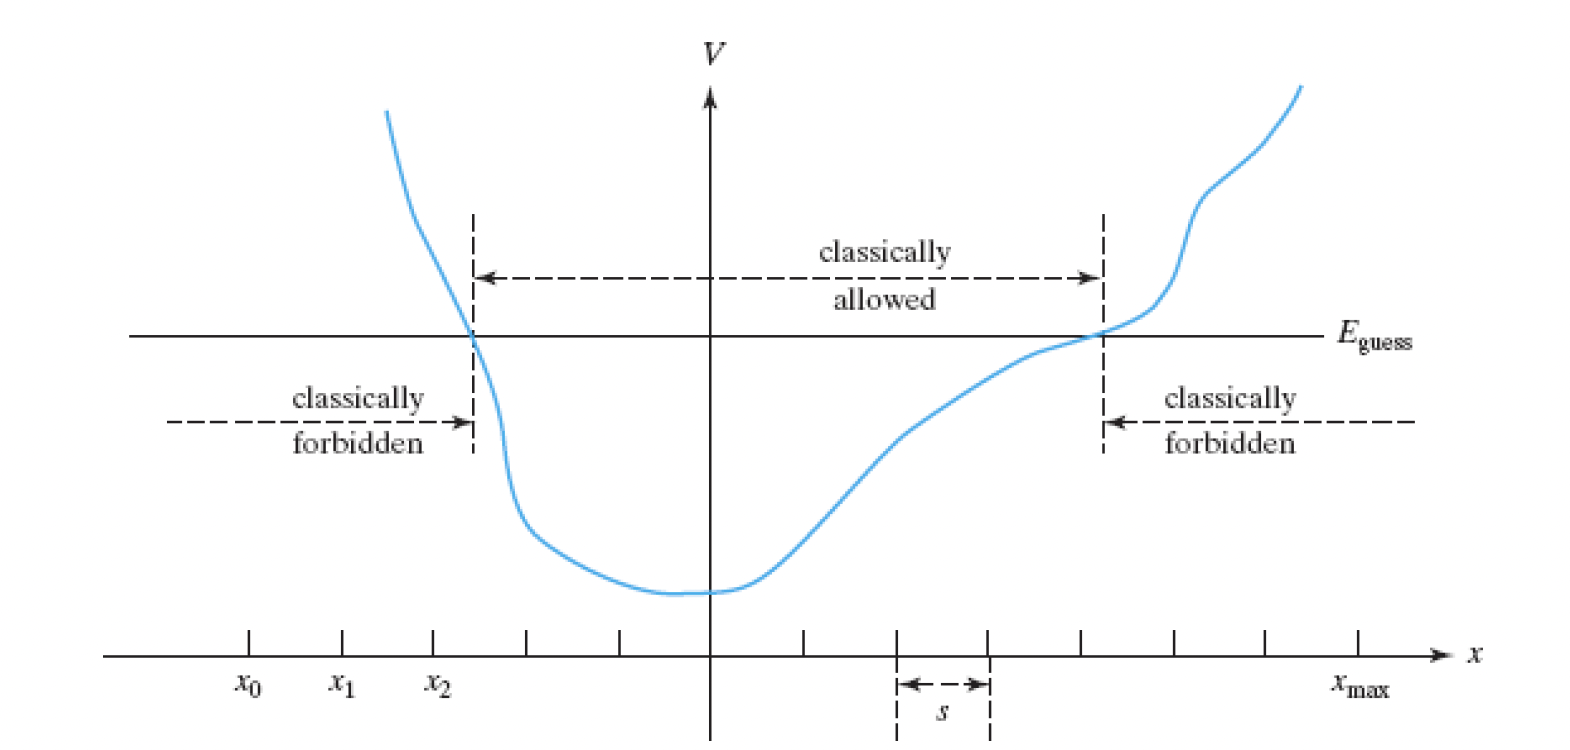
\includegraphics[width=0.8\textwidth]{figures/4.7.png}
        \caption{一维单粒子系统的$V$关于$x$的图象}
        \label{fig:4.7}
    \end{figure}
    \\
    \indent 用涉及$s$的幂的Taylor级数展开$\psi\left(x_n+s\right)$和$\psi\left(x_n-s\right)$,将两式相加即可消去$s$的奇次幂项,并用薛定谔方程来表示 $\psi^{\prime\prime}$ 和 $\psi^{\left(\mathrm{iv}\right)}$,以 $\psi$ 表示,并忽略 $s^6$ 和 $s$ 的高次幂项(如果 $s$ 较小,近似值将是准确的),我们会发现(问题 4.43)
    \begin{equation}
        \psi_{n+1} \equiv = \frac{
            2\psi_n - \psi_{n-1} + 5G_n\psi_n s^2/6 + G_{n-1}\psi_{n-1}s^2/12
        }{
            1-G_{n+1}s^2/12
        }
        \label{eq:4.67}
    \end{equation}
    其中$G_n \equiv G\left(x_n\right) \equiv m\hbar^{-2}\left[2V\left(x_n\right)-2E\right]$[式(\ref{eq:4.66})和\ref{eq:4.65}]。如果知道$\psi_n$和$\psi_{n-1}$,即$\psi$在$x_n$和$x_n-s$处的值,方程(\ref{eq:4.67})允许我们计算$\psi_{n+1}$,即$\psi$在点$x_{n+s}$处的值。\\
    \indent 我们如何使用式(\ref{eq:4.67})来求解薛定谔方程?我们首先猜测一个能量本征值$E_{guess}$。我们从左侧经典禁区(图 \ref{fig:4.7})中的一点 $x_0$ 开始,此处$\psi$的值很小,我们假设$\psi$在该点处的值为零:$\psi_0 \equiv \psi\left(x_0\right) = 0$。同样地,我们也在经典禁区(此处$\psi$的值也很小)的右侧点 $x_{max}$ 处假设 $\psi\left(x_{max}\right)$ 的值为零。我们为连续点之间的间隔 $s$ 选取一个较小的数值,在$x_0+s$处,我们将$\psi$的值设为一个较小的数值,例如0.0001:$\psi_1 \equiv \psi\left(x_1\right) \equiv \psi\left(x_0+s\right) = 0.0001$。$\psi_1$ 的值对找到的本征值不会有任何影响。如果我们令$\psi_1$为0.001,而不是0.0001,公式 (\ref{eq:4.67}) 表明,这只需将后续点上的所有 $\psi$ 值乘以 10 即可(问题 4.41)。这不会影响本征值[见公式 (\ref{eq:3.14 definition of eigenfunctions and eigenvalues}) 后的示例]。在找到每个本征值后,可以对波函数进行归一化处理。\\
    \begin{figure}[h!]
        \centering
        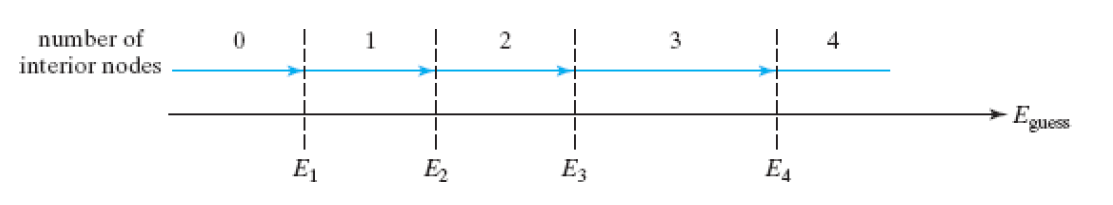
\includegraphics[width=0.8\textwidth]{Figures/4.8.png}
        \caption{Numerov 方法求解的节点数与能量 $E_{guess}$ 的函数关系。}
        \label{fig:4.8}
    \end{figure}\\
    \indent 现在我们有了 $\psi_0$ 和 $\psi_1$ 的值,可以使用式 (\ref{eq:4.67}) 计算 $\psi_2 \equiv \psi\left(x_2\right) \equiv \psi\left(x_1+2s\right)$ 的值,其中我们用$E_{guess}$计算得到$G$的值。接着,在式(\ref{eq:4.67})令$n=2$,我们可以计算出$\psi_3$的值,以此类推,直到达到$x_{max}$。如果$E_{guess}$不等于或不非常接近于本征值,那么$\psi$将不满足平方可积的要求,且$\left|\psi\left(x_{max}\right)\right|$的值会变得非常大。如果发现$\left|\psi\left(x_{max}\right)\right|$不接近于零,那我们重新选一个$E_{guess}$,并从$x_0$开始重复上述过程。这个过程将会循环往复,直到找到能使$\left|\psi\left(x_{max}\right)\right|$非常接近于零的$E_{guess}$的值。此时的$E_{guess}$基本上等同于一个本征值。找到本征值的系统方法是计算由 $E_{guess}$ 生成的 $\psi$ 中的节点。回忆在一维问题中(第\ref{sec:4.2 The One-Dimensional Harmonic Oscillator}节),基态的内部节点数为 0,第一激发态的内部节点数为 1,以此类推。令$E_1,E_2,E_3,\cdots$分别表示基态、第一激发态和第二激发态等的能量值。如果$\psi_{guess}$在$x_0$和$x_{max}$之间没有节点,那么$E_{guess}$应该小于或等于$E_1$。如果$\psi_{guess}$在$x_0$和$x_{max}$之间有一个节点,那么$E_{guess}$应该位于$E_1$和$E_2$之间。随后将给出例子。\\
    \\
    \noindent\textbf{无量纲变量}\\
    \indent Numerov方法需要我们猜测$E$的值。但是我们猜测的数量级:$10^{-20} \: \mathrm{J},10^{-15} \: \mathrm{J},\cdots$应该是多少?为了回答这个问题,我们以谐振子为例,用无量纲变量重表示薛定谔方程。\\
    \indent 谐振子的势能函数为$V = \frac{1}{2}kx^2$,其薛定谔方程包含三个常数,$k$、$m$和$\hbar$。我们试图找到无量纲约化能量 $E_r$ 和无量纲约化 $x$ 坐标 $x_r$,它们的定义是
    \begin{equation}
        E_r \equiv E/A, \quad x_r \equiv x/B
        \label{eq:4.68}
    \end{equation}
    其中常数$A$是$k$、$m$和$\hbar$的组合,具有能量的量纲,而$B$是具有长度量纲的组合。能量的量纲为$\text{质量}\times\text{长度}^2\times\text{时间}^{-2}$,我们写作
    \begin{equation}
        \left[E\right] = \mathrm{M}\mathrm{L}^2\mathrm{T}^{-2}
        \label{eq:4.69}
    \end{equation}
    其中,$E$ 的括号表示其维度,$\mathrm{M}$、$\mathrm{L}$ 和 $\mathrm{T}$ 分别表示质量、长度和时间。方程$V = \frac{1}{2}kx^2$表明$k$的量纲为$\text{能量}\times\text{长度}^{-2}$,由式(\ref{eq:4.69}),有$\left[k\right] = \mathrm{M}\mathrm{T}^{-2}$。$\hbar$的量纲为$\text{能量}\times\text{时间}$。因此,
    \begin{equation}
        \left[m\right] = \mathrm{M}, \quad \left[k\right] = \mathrm{M}\mathrm{T}^{-2}, \quad \left[\hbar\right] = \mathrm{M}\mathrm{L}^2\mathrm{T}^{-1}
        \label{eq:4.70}
    \end{equation}
    式(\ref{eq:4.68})中的$A$和$B$的量纲分别为能量和长度,则
    \begin{equation}
        \left[A\right] = \mathrm{M}\mathrm{L}^2\mathrm{T}^{-2}, \quad \left[B\right] = \mathrm{L}
        \label{eq:4.71}
    \end{equation}
    \indent 令$A = m^ak^b\hbar^c$,其中$a$、$b$和$c$是待定的指数,由$A$的量纲一定为$\mathrm{M}\mathrm{L}^2\mathrm{T}^{-2}$所确定。我们有
    \begin{equation}
        \left[A\right] = \left[m^ak^b\hbar^c\right] = \mathrm{M}^a\left(\mathrm{M}\mathrm{T}^{-2}\right)^b\left(\mathrm{M}\mathrm{L}^2\mathrm{T}^{-1}\right)^c = \mathrm{M}^{a+b+c}\mathrm{L}^{2c}\mathrm{T}^{-2b-c}
        \label{eq:4.72}
    \end{equation}
    令 (\ref{eq:4.71}) 和 (\ref{eq:4.72}) 中 M、L 和 T 的指数相等,得到
    \begin{equation*}
        a+b+c = 1, \quad 2c = 2, \quad -2b-c = -2
    \end{equation*}
    解这个方程组,得到$c=1$,$b=\frac{1}{2}$,$a=-\frac{1}{2}$。因此
    \begin{equation}
        A = m^{-1/2}k^{1/2}\hbar
        \label{eq:4.73}
    \end{equation}
    \indent 同样地,令$B = m^dk^e\hbar^f$。用得出式(\ref{eq:4.73})相同的量纲分析法,有(问题4.44)
    \begin{equation}
        B = m^{-1/4}k^{-1/4}\hbar^{1/2}
        \label{eq:4.74}
    \end{equation}
    \indent 根据式(\ref{eq:4.68})、(\ref{eq:4.73})和(\ref{eq:4.74}),谐振子的约化变量为
    \begin{equation}
        E_r = E / m^{-1/2}k^{1/2}\hbar, \quad x_r = x / m^{-1/4}k^{-1/4}\hbar^{1/2}
        \label{eq:4.75}
    \end{equation}
    使用$k^{1/2} = 2\pi\nu m^{1/2}$[式(\ref{eq:4.23})]将$k$从(\ref{eq:4.75})中消去,并回忆$\alpha \equiv 2\pi\nu m/\hbar$[式(\ref{eq:4.31})],我们得到以下备选的表达式
    \begin{equation}
        E_r = E /h\nu, \quad x_r = \alpha ^{1/2}x
        \label{eq:4.76}
    \end{equation}
    \indent 与方程$E_r \equiv E/A$[式(\ref{eq:4.68})]类似,我们可以定义约化势能函数$V_r$:
    \begin{equation}
        V_r \equiv V / A
        \label{eq:4.77}
    \end{equation}
    \indent 由于$\left|\psi\left(x\right)\right|^2\mathrm{d}x$是概率,概率是没有量纲的,归一化后的$\psi\left(x\right)$一定具有$\text{长度}^{-1/2}$的量纲。因此,我们可以定义一个没有量纲的约化波函数$\psi_r$。由式(\ref{eq:4.71}),$B$具有长度的量纲,则$B^{-1/2}$具有$\text{长度}^{-1/2}$的量纲。因此,
    \begin{equation}
        \psi_r = \psi / B^{-1/2}
        \label{eq:4.78}
    \end{equation}
    $\psi_r$ 满足 $\int_{-\infty}^{\infty} \left|\psi_r\right|^2\mathrm{d}x_r = 1$;这是由式(\ref{eq:4.76})、 (\ref{eq:4.78}) 和$\int_{-\infty}^{\infty} \left|\psi\right|^2\mathrm{d}x = 1$得出的。\\
    \indent 我们现在使用无量纲变量$E_r$、$x_r$和$\psi_r$来重写薛定谔方程。有
    \begin{equation*}
        \frac{\mathrm{d}^2\psi}{\mathrm{d}x^2} = \frac{\mathrm{d}^2}{\mathrm{d}x^2}B^{-1/2}\psi_r = B^{-1/2}\frac{\mathrm{d}}{\mathrm{d}x}\frac{\mathrm{d}\psi_r}{\mathrm{d}x} = B^{-1/2}\frac{\mathrm{d}}{\mathrm{d}x}\frac{\mathrm{d}\psi_r}{\mathrm{d}x_r}\frac{\mathrm{d}x_r}{\mathrm{d}x} = B^{-1/2}\frac{\mathrm{d}\left(\mathrm{d}\psi_r/\mathrm{d}x_r\right)}{\mathrm{d}x_r}\frac{\mathrm{d}x_r}{\mathrm{d}x}\frac{\mathrm{d}x_r}{\mathrm{d}x}
    \end{equation*}
    \begin{equation}
        \frac{\mathrm{d}^2\psi}{\mathrm{d}x^2} = B^{-5/2}\frac{\mathrm{d}^2\psi_r}{\mathrm{d}x_r^2}
        \label{eq:4.79}
    \end{equation}
    其中,我们用到了$\mathrm{d}x_r/\mathrm{d}x = B^{-1/2}$。将式(\ref{eq:4.68})、(\ref{eq:4.77})和(\ref{eq:4.79})代入薛定谔方程$-\left(\hbar^2/m\right)\left(\mathrm{d}^2\psi/\mathrm{d}x^2\right) + V\psi = E\psi$,得到
    \begin{equation*}
        -\frac{\hbar^2}{m}B^{-5/2}\frac{\mathrm{d}^2\psi_r}{\mathrm{d}x_r^2} + AV_rB^{-1/2}\psi_r = AE_rB^{-1/2}\psi_r
    \end{equation*}
    \begin{equation}
        -\frac{\hbar^2}{2m}\frac{1}{AB^2}\frac{\mathrm{d}^2\psi_r}{\mathrm{d}x_r^2} + V_r\psi_r = E_r\psi_r
        \label{eq:4.80}
    \end{equation}
    根据式(\ref{eq:4.73})和(\ref{eq:4.74}),有$AB^2 = \hbar^2/m$,所以对于谐振子,有$\hbar^2/mAB^2 = 1$。\\
    \indent 更一般地说,让 $V$ 包含一个非无量纲参数 $c$。例如,我们有$V = cx^4$或$V = cx^2\left(1+0.05m^{1/2}c^{1/2}\hbar^{-1}x^2\right)$(注意 $m^{1/2}c^{1/2}\hbar^{-1}x^2$ 是无量纲的,因为 1 是无量纲的,所以它必须是无量纲的)。式(\ref{eq:4.80})中的$AB$一定可以写成$\hbar^rm^sc^t$的形式,其中$r$、$s$和$t$是待定的指数。由于(\ref{eq:4.80})中的$V_r\psi_r$是无量纲的,因此第一项也是无量纲的。那么$\hbar^2/mAB^2$是无量纲的,$AB^2$与$\hbar^2/m$具有相同的量纲。所以$r=2$,$s=1$,$t=0$。因此,$AB^2 = \hbar^2/m$,带入(\ref{eq:4.80}),有无量纲的薛定谔方程
    \begin{equation}
        \frac{\mathrm{d}^2\psi}{\mathrm{d}x_r^2} = \left(2V_r-2E_r\right)\psi_r
        \label{eq:4.81}
    \end{equation}
    \begin{equation}
        \psi^{\prime\prime} = G_r\psi_r, \quad \text{其中} \quad G_r \equiv 2V_r-2E_r
        \label{eq:4.82}
    \end{equation}
    对于谐振子,$V_r \equiv V/A = \frac{1}{2}kx^2/m^{-1/2}k^{1/2}\hbar = \frac{1}{2}x_r^2$,因此[式(\ref{eq:4.73})和式(\ref{eq:4.75})]:
    \begin{equation}
        V_r = \frac{1}{2}x_r^2
        \label{eq:4.83}
    \end{equation}
    \indent 将谐振子薛定谔方程约化为只涉及无量纲量的形式 (\ref{eq:4.81})后,我们可以预期最低能量本征值的数量级为 1。\\
    \indent 约化谐振子薛定谔方程(\ref{eq:4.82})与(\ref{eq:4.66})具有相同的形式,所以我们可以用Numerov公式(\ref{eq:4.67})来求解。使用$\psi_r$的值代替$\psi$,$G_r$的值代替$G$,与(\ref{eq:4.68})类似,$s_r$的值代替$s$。\\
    \indent 一旦找到约化能量$E_r$的数值,就可以根据 (\ref{eq:4.75}) 或 (\ref{eq:4.76}) 求出能量 $E$。\\
    \\
    \textbf{$x_r$、$x_0$ 、 $x_{max}$ 和$s_r$的选择}\\
    \indent 我们需要选择$x_r$的起始值、结束值,以及相邻点之间的间隔值$s_r$。假设我们希望找到满足$E_r \le 5$的谐振子的所有本征函数和本征值。我们从左侧经典禁区开始求解,因此首先要找到 $E_r=5$ 的经典禁区。经典允许和经典禁止区域的边界满足$E_r=V_r$。由式(\ref{eq:4.83}),有$V_r = \frac{1}{2}x_r^2$,因此$E_r=V_r$变成了$5=\frac{1}{2}x_r^2$所以满足$E_r \le 5$的经典允许区域为$x_r = -\left(10\right)^{1/2}=-3.16$到$x_r = \left(10\right)^{1/2}=3.16$。若$E_r<5$,则经典允许区域将更小。我们希望从左侧经典禁区($\psi$ 非常小)内的某一点开始求解,我们希望在右侧经典禁区内的某一点结束求解。对于$E_r=5$,左侧的经典禁区在$x_r=-3.16$处结束,,所以一个合理的选择为$x_r=-5$[太深入经典禁区有时会带来麻烦(见下文),因此在选择起点时可能需要试错]。由于 $V$ 是对称的,因此我们将在 $x_r=5$ 处结束求解。\\
    \indent 为了达到合理的精确度,通常至少需要 100 个点,因此我们取 $s_r=0.1$ 以得到 100 个点。从 Numerov 方法的推导中可以看出,$s_r$ 必须很小。合理的规则可能是 $s_r$ 不大于 0.1。
    \begin{quote}
        \small
        \noindent
        如果像通常情况那样,当$x \to \pm \infty$时有$V \to \infty$,那么在经典禁区内起步太远会使 Numerov 公式 (\ref{eq:4.67}) 中的分母 $1-G_{n+1}s^2/12$ 变成负数。我们有 $G_r=2V_r-2E_r$,如果我们从 $V_r$ 非常大的点 $x_0$ 开始,该点的 $G_r$ 可能大到足以使 Numerov 公式的分母为负。这样,该方法就会失效。我们将 $\psi_0$ 取为零,将 $\psi_1$ 取为正数。Numerov 公式 (\ref{eq:4.67}) 表明,如果分母是负数,那么 $\psi_2$ 也将是负数,我们将在 $x_1$ 和 $x_2$ 之间产生一个虚假的 $\psi$ 节点。为了避免这个问题,我们可以减小步长 $s_r$ 或 $x_r$、$x_{max}$、$-x_r$和$-x_0$。(见问题 4.46)。
    \end{quote}

    \noindent\textbf{Numerov方法的计算机程序}

    \noindent\textbf{使用电子表格求解一维薛定谔方程}

    \noindent\textbf{Numerov 方法步骤摘要}






    



\section*{总结}

\section*{习题}
